% Research poster, DIN A1 portrait (594 x 841 mm).
% Empirical work: own replication of the wisdom-of-crowds Turing Experiment (Aher et al. 2023) with Qwen2.5-0.5B.
% Every number is traceable: literature numbers -> % SOURCE comments (page/table of the cited paper);
% experiment numbers -> macros generated by experiment/analyze.py (results/numbers.tex, results/summary.json).
\documentclass[final]{beamer}
\usepackage[size=custom,width=59.4,height=84.1,scale=1.0]{beamerposter}
\usepackage[utf8]{inputenc}
\usepackage[T1]{fontenc}
\usepackage{lmodern}
\usepackage{graphicx}
\usepackage{booktabs}
\usepackage[most]{tcolorbox}
\usepackage{tikz}
\usetikzlibrary{arrows.meta}

% generated by analyze.py from results/summary.json -- do not edit
\newcommand{\xBaseExact}{4.0\,\%}
\newcommand{\xBaseExactCI}{2.4\,\%--5.8\,\%}
\newcommand{\xBaseNExact}{20}
\newcommand{\xBaseNValid}{497}
\newcommand{\xBaseNIQR}{1.23}
\newcommand{\xBaseNIQRfive}{1.68}
\newcommand{\xBaseIQRzero}{0}
\newcommand{\xBaseRelErr}{0.87}
\newcommand{\xInstExact}{1.4\,\%}
\newcommand{\xInstExactCI}{0.4\,\%--2.6\,\%}
\newcommand{\xInstNExact}{7}
\newcommand{\xInstNValid}{500}
\newcommand{\xInstNIQR}{5.53}
\newcommand{\xInstNIQRfive}{6.64}
\newcommand{\xInstIQRzero}{0}
\newcommand{\xInstRelErr}{0.91}
\newcommand{\xChatExact}{1.0\,\%}
\newcommand{\xChatExactCI}{0.2\,\%--1.8\,\%}
\newcommand{\xChatNExact}{5}
\newcommand{\xChatNValid}{500}
\newcommand{\xChatNIQR}{0.41}
\newcommand{\xChatNIQRfive}{0.82}
\newcommand{\xChatIQRzero}{0}
\newcommand{\xChatRelErr}{0.77}
\newcommand{\xHumNIQRfive}{0.81}
\newcommand{\xInstFisherP}{$p=0.011$}
\newcommand{\xInstFisherOR}{0.3}
\newcommand{\xInstWilcP}{$p=0.020$}
\newcommand{\xInstLower}{2}
\newcommand{\xChatFisherP}{$p=0.002$}
\newcommand{\xChatFisherOR}{0.2}
\newcommand{\xChatWilcP}{$p=0.037$}
\newcommand{\xChatLower}{9}

% Public repository with code + raw outputs (REQUIRED by the poster rules). Replace the red text by the URL:
% \newcommand{\repourl}{github.com/<user>/<repo>}
\newcommand{\repourl}{{\fsSmall github.com/ssowrabha249-coder/\\\mbox{Simulating-Voices-and-Fabricating-Realities-{}-Poster}}}

\setbeamertemplate{navigation symbols}{}
\tikzset{box/.style={draw=#1, line width=1.5pt, fill=#1!8, rounded corners=3mm, align=center, inner sep=4mm},
  arr/.style={-{Latex[length=5mm]}, line width=2pt, black!60}}

% Font sizes at print size (poster is printed at 100 %). Nothing below 24 pt.
\newcommand{\fsBody}{\fontsize{26}{32}\selectfont}
\newcommand{\fsSmall}{\fontsize{24.2}{29}\selectfont}% 24.2 TeX pt = 24.1 PDF pt (TeX pt is 1/72.27 in)
\newcommand{\fsSub}{\fontsize{30}{36}\selectfont\bfseries}
\newcommand{\fsSec}{\fontsize{42}{50}\selectfont\bfseries}
\newcommand{\fsTitle}{\fontsize{68}{78}\selectfont\bfseries}
\newcommand{\fsKey}{\fontsize{80}{84}\selectfont\bfseries}

\definecolor{navy}{RGB}{16, 42, 77}
\definecolor{teal}{RGB}{13, 118, 110}
\definecolor{sand}{RGB}{255, 247, 214}
\definecolor{ink}{RGB}{20, 27, 40}
\definecolor{cbase}{HTML}{6B7785}
\definecolor{cinst}{HTML}{1F5F8B}
\definecolor{cchat}{HTML}{0D766E}
\definecolor{chum}{HTML}{B35F00}
\setbeamercolor{background canvas}{bg=white}
\setbeamercolor{normal text}{fg=ink}

\tcbset{
  sec/.style={enhanced, colback=white, colframe=navy, boxrule=2.5pt, arc=4mm,
    left=10mm, right=10mm, top=11mm, bottom=7mm, fonttitle=\fsSec, coltitle=white, colbacktitle=navy,
    attach boxed title to top left={xshift=10mm, yshift=-5mm}, boxed title style={arc=3mm, boxrule=0pt, left=6mm, right=6mm, top=2mm, bottom=2mm}},
  card/.style={enhanced, colback=navy!4, colframe=navy!25, boxrule=1.2pt, arc=3mm, left=7mm, right=7mm, top=4mm, bottom=4mm},
  key/.style={enhanced, colback=#1!8, colframe=#1, boxrule=2pt, arc=3mm, left=5mm, right=5mm, top=3mm, bottom=3mm, halign=center, valign=top},
  take/.style={enhanced, colback=sand, colframe=orange!70!black, boxrule=2.5pt, arc=4mm, left=10mm, right=10mm, top=5mm, bottom=5mm}
}
\renewcommand{\cite}[1]{{\color{navy!80}[#1]}}

\begin{document}
\begin{frame}[t]
\vspace{-6mm}

% ------------------------------------------------------------------ HEADER
\begin{tcolorbox}[enhanced, colback=navy, colframe=navy, arc=5mm, left=15mm, right=15mm, top=5mm, bottom=5mm, halign=center]
  {\fontsize{28}{34}\selectfont\color{white!80} Universität Trier $\cdot$ Fachbereich II $\cdot$ Computational Linguistics $\cdot$ M.Sc.\ Natural Language Processing}\\[3mm]
  {\fsTitle\color{white} Simulating Voices: Does Instruction Tuning Make a Simulated Crowd Hyper-Accurate?}\\[3mm]
  {\fontsize{36}{44}\selectfont\color{teal!25} A replication of the wisdom-of-crowds Turing Experiment with an open base\,/\,instruct LLM pair}\\[5mm]
  {\fontsize{30}{36}\selectfont\color{white} \textbf{Sowrabha Somashekar} \quad$\cdot$\quad Matr.\ 1837734 \quad$\cdot$\quad s2sosoma@uni-trier.de \quad$\cdot$\quad Supervisor: Dr. phil. Simon Werner}
\end{tcolorbox}

\vspace{3mm}

% ------------------------------------------------------------------ ROW 1
\begin{columns}[T]
\begin{column}{0.485\linewidth}

\begin{tcolorbox}[sec, title={1. Hypothesis}]
\fsBody
\textbf{Context.} LLMs serve as \emph{synthetic participants} in behavioural and opinion research \cite{Aher; Santurkar}. This only works if simulated people show \emph{human-like variation}.

\vspace{4mm}
\begin{tcolorbox}[card]
{\fsSub\color{navy} Prior work: the hyper-accuracy distortion}\\[2mm]
Asked ``How many bones does an adult human have?'', humans answer with median 190 (IQR 108); GPT-4 answers 206, the exact value, with IQR 0 \cite{Aher, Tab.\,3--4}.
% SOURCE: Aher et al. Table 3 p.25 (human 190, IQR 108), Table 4 p.26 (gpt-4 206, IQR 0)
Aher et al.\ suspect alignment as the cause, but could only test closed models whose training details are not released \cite{Aher, p.\,25}.
% SOURCE: Aher et al. p.25 ("specific details of the LMs in question have not been released"); p.3 ("may be due to alignment")
\end{tcolorbox}

\vspace{4mm}
\begin{tcolorbox}[card]
{\fsSub\color{navy} Research question \& hypothesis}\\[2mm]
\textbf{RQ} Does instruction tuning \emph{alone} make a simulated crowd give exact answers without human-like spread?\\[2mm]
\textbf{H1} With the \emph{same prompt}, an instruction-tuned model gives
(a)~\textbf{more exact answers} and (b)~a \textbf{smaller spread} than its base model.\\[2mm]
\textbf{Contribution:} a test with an open model pair in which only post-training differs.
\end{tcolorbox}
\end{tcolorbox}

\end{column}
\begin{column}{0.485\linewidth}

\begin{tcolorbox}[sec, title={2. Methodology}]
\fsBody
\begin{tcolorbox}[card]
{\fsSub\color{navy} Design}\\[2mm]
\textbf{Models:} Qwen2.5-0.5B vs.\ Qwen2.5-0.5B-Instruct \cite{Qwen Team}.\\[1mm]
\textbf{Data:} 10 questions with true values; human median/IQR for Q1--5 \cite{Aher, Tab.\,3}.\\[1mm]
\textbf{Crowd:} 50 simulated people (25 surnames $\times$ Mr./Ms.) per question.\\[1mm]
\textbf{Prompt \& sampling} as Aher et al.: Fig.\,14, temperature 1, top-$p$ 1; invalid answers re-sampled.
% SOURCE: Aher et al. Table 3 p.25; Fig. 14 p.25; p.7 (temperature = 1, top p = 1)
\end{tcolorbox}

\vspace{4mm}
\centering
\begin{tikzpicture}[font=\fsSmall]
  \node[box=navy, text width=24cm] (in) at (0,0) {\textbf{10 questions $\times$ 50 simulated people} $\to$ Aher et al.\ prompt};
  \node[box=cbase, text width=7.4cm] (c1) at (-8.4,-2.6) {\textbf{base}\\ same prompt};
  \node[box=cinst, text width=7.4cm] (c2) at ( 0.0,-2.6) {\textbf{instruct}\\ same prompt};
  \node[box=cchat, text width=7.4cm] (c3) at ( 8.4,-2.6) {\textbf{instruct}\\ chat template};
  \node[box=navy, text width=24cm] (m) at (0,-5.9) {\textbf{Measures:} exact answers (bootstrap 95\,\% CI); spread = IQR\,/\,true value.
    \textbf{Tests} vs.\ base: Fisher exact (a), Wilcoxon over 10 questions (b); Bonferroni $\alpha{=}0.0125$};
  \foreach \c in {c1,c2,c3} { \draw[arr] (in.south) -- ++(0,-0.4) -| (\c.north); \draw[arr] (\c.south) -- (\c.south |- m.north); }
\end{tikzpicture}

\vspace{2mm}
\raggedright
\begin{tcolorbox}[card, top=2mm, bottom=2mm]
{\fsSub\color{navy} Code \& all 1,500 raw outputs:}\\ \repourl
\end{tcolorbox}
\end{tcolorbox}

\end{column}
\end{columns}

\vspace{3mm}

% ------------------------------------------------------------------ RESULTS (full width)
\begin{tcolorbox}[sec, title={3. Results}]
\fsBody
\centering
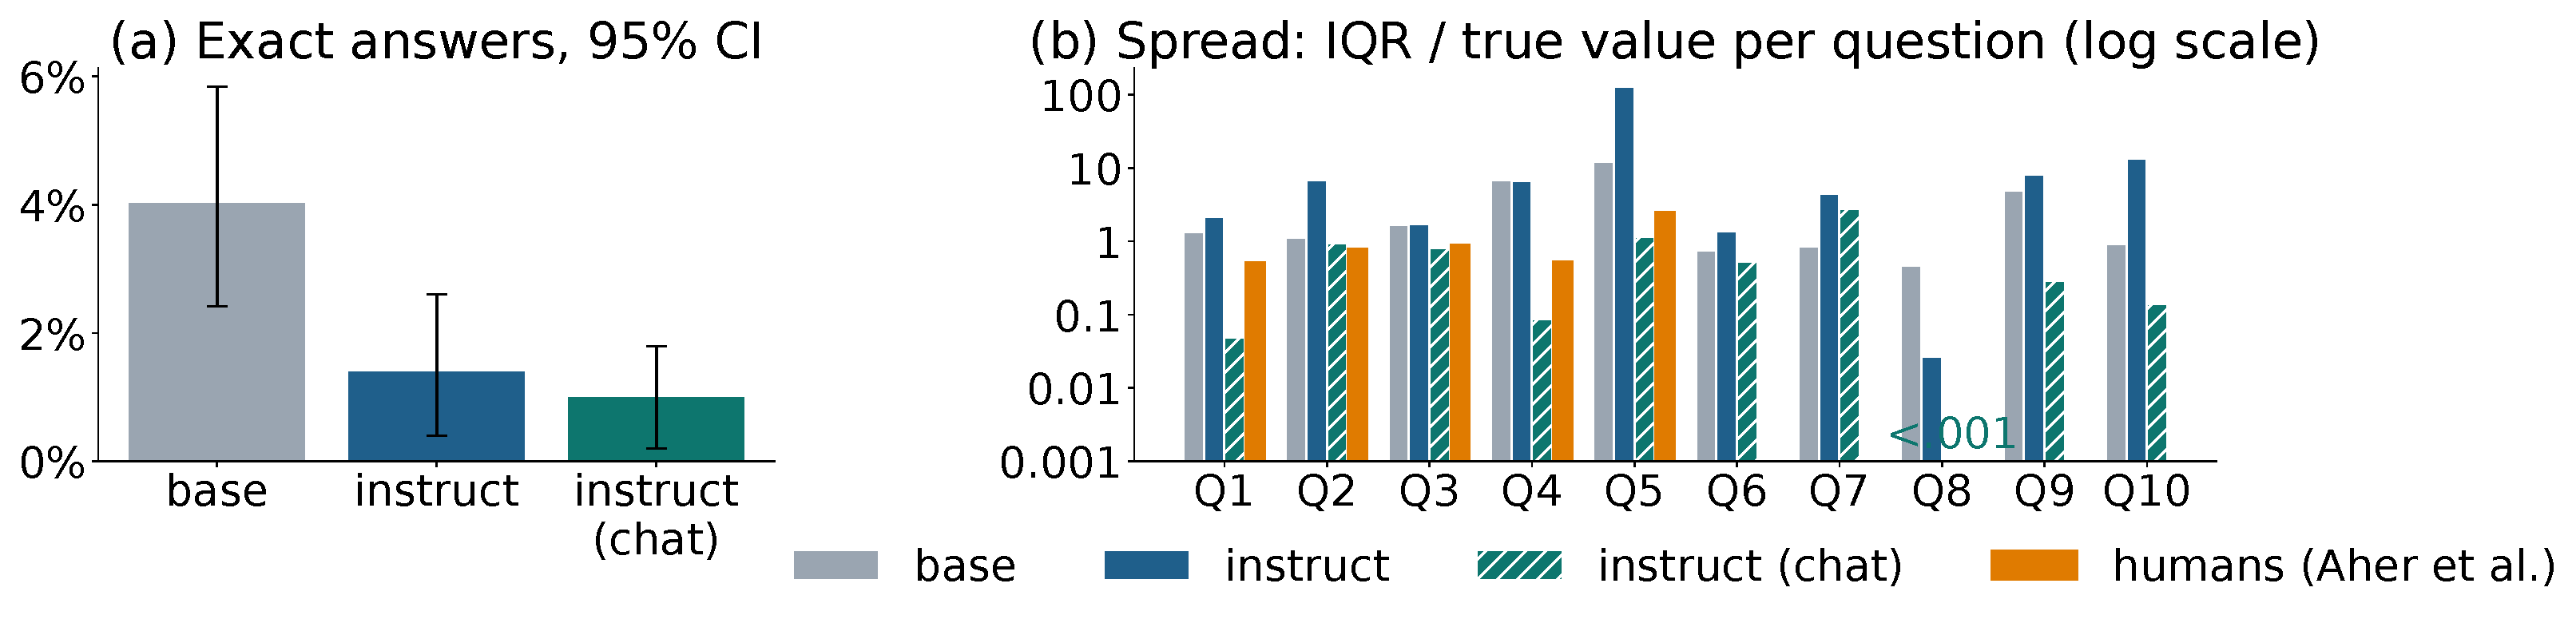
\includegraphics{experiment/results/figures/fig_crowd_poster.pdf}\\[1mm]
\raggedright
{\fsSmall \textbf{Figure.} (a) Pooled share of exactly correct answers, 95\,\% bootstrap CI. (b) IQR / true value per question (log scale); human values from Aher et al., Tab.\,3 (Q1--Q5 only). Q8 (speed of light, 299,792,458): the ratio is tiny for all conditions and does not mean accurate answers.}

\vspace{5mm}
\begin{columns}[T]
\begin{column}{0.47\linewidth}
{\fsSub\color{navy} Summary per condition}\\[2mm]
\fsSmall
\begin{tabular}{@{}lccc@{}}
\toprule
 & \textbf{exact (95\,\% CI)} & \textbf{spread} & \textbf{spread Q1--5}\\
\midrule
base & \xBaseExact{} (\xBaseExactCI) & \xBaseNIQR & \xBaseNIQRfive\\
instruct & \xInstExact{} (\xInstExactCI) & \xInstNIQR & \xInstNIQRfive\\
instr.\ (chat) & \xChatExact{} (\xChatExactCI) & \xChatNIQR & \xChatNIQRfive\\
humans & -- & -- & \xHumNIQRfive\\
\bottomrule
\end{tabular}\\[2mm]
spread = median over questions of IQR / true value.

\vspace{4mm}
{\fsSub\color{navy} Interpretation}\\[2mm]
\fsBody hyper-accuracy may need alignment \emph{plus} the knowledge of larger models; Aher et al.'s smallest models did not show it either \cite{Aher, Tab.\,3}.
% SOURCE: Aher et al. Table 3 p.25 (LM-1 to LM-3 medians far from truth)
\end{column}
\begin{column}{0.49\linewidth}
{\fsSub\color{navy} Discussion vs.\ hypothesis}\\[2mm]
\textbf{H1(a) not supported, opposite direction:} both instruct conditions give \emph{fewer} exact answers than base (Fisher \xInstFisherP, \xChatFisherP; significant after correction). No condition has IQR\,=\,0 on any question (GPT-4: all 10 \cite{Aher, Tab.\,4}).
% SOURCE: Aher et al. Table 4 p.26 (gpt-4 IQR 0 on all 10 questions); own: n_questions_iqr0 = 0 in summary.json
\\[2mm]
\textbf{H1(b) not supported:} same prompt $\Rightarrow$ \emph{more} spread on \the\numexpr10-\xInstLower\relax{} of 10 questions (\xInstWilcP, n.s.\ after correction).\\[2mm]
\textbf{Unexpected:} the chat format narrows the spread (\xChatLower{}/10 questions, \xChatWilcP, n.s.); Q1--5 close to humans (\xChatNIQRfive{} vs.\ \xHumNIQRfive) but around \emph{wrong} values (median: 24 bones).
% SOURCE: experiment/results/tables/per_question.csv (instruct_chat q01 median 24.0)

\vspace{4mm}
{\fsSub\color{navy} Limitations}\\[2mm]
\fsSmall One model size (0.5B), one prompt wording, 10 questions; human values taken from Aher et al., not collected; spread ratio is misleading for Q8.
\end{column}
\end{columns}

\vspace{4mm}
\begin{tcolorbox}[take]
{\fsSub\color{orange!50!black} Take-home:} \fsBody instruction tuning alone did \textbf{not} make a small simulated crowd hyper-accurate. Check spread and correctness \textbf{separately}; next: repeat across model sizes.
\end{tcolorbox}

\vspace{1mm}
{\fsSmall Full references, AI-use statement and the signed declaration are in the appendix PDF.}
\end{tcolorbox}

\end{frame}
\end{document}
